% The three-way handshake: Propagator stepping loop mediates between
% Navigator (geometry) and CKF Actor (measurements).
% Reference: Acts/Propagator/Propagator.ipp:99-193
\documentclass[border=8pt]{standalone}
\usepackage{tikz}
\usepackage{newtxtext,newtxmath}
\usetikzlibrary{arrows.meta,positioning,calc,fit,backgrounds}

\begin{document}
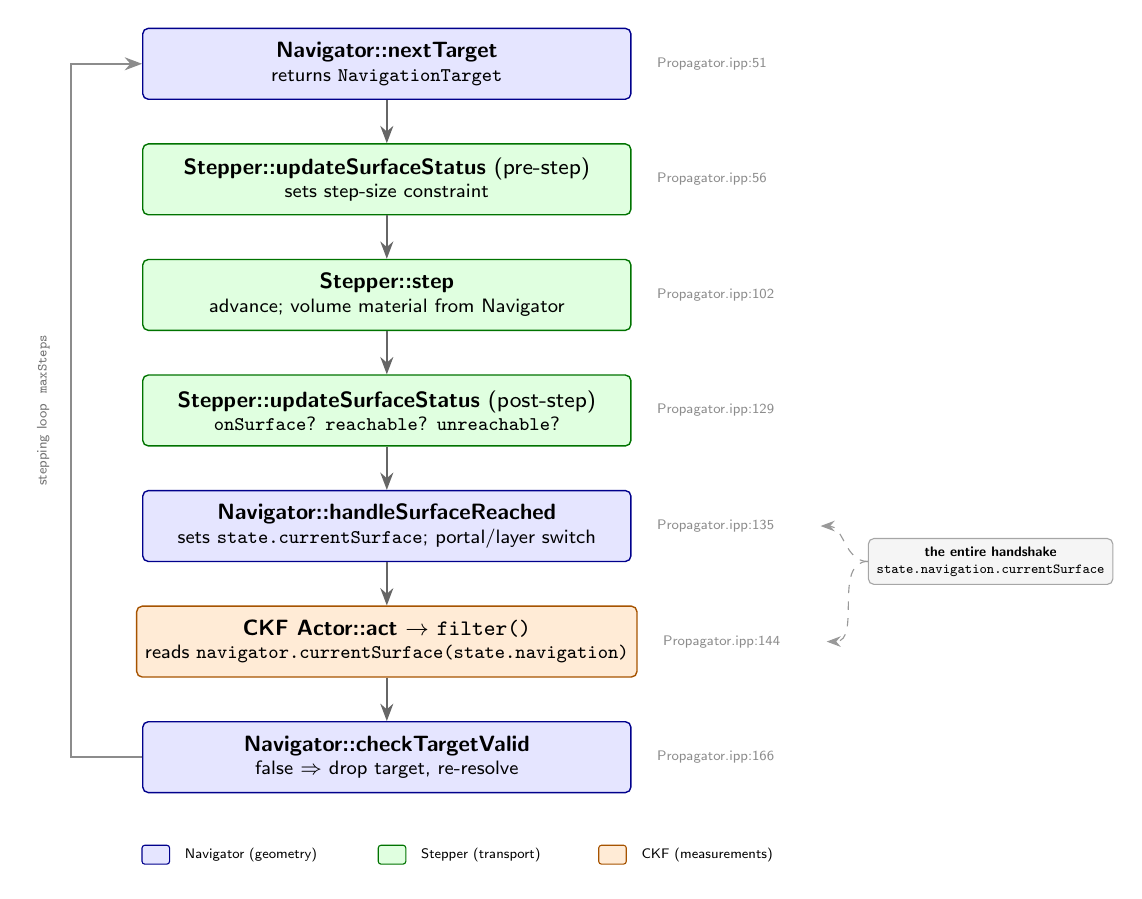
\begin{tikzpicture}[
  font=\sffamily\footnotesize,
  box/.style={rounded corners=2pt,draw,minimum width=62mm,minimum height=9mm,
              align=center,inner sep=3pt,line width=0.5pt},
  nav/.style ={box,fill=blue!10,draw=blue!55!black},
  stp/.style ={box,fill=green!12,draw=green!45!black},
  act/.style ={box,fill=orange!16,draw=orange!65!black},
  fl/.style={-{Stealth[length=2.2mm]},line width=0.7pt,draw=black!60},
  ref/.style={font=\sffamily\tiny,text=black!45,anchor=west}
]

\node[nav] (n1) at (0,0)
  {\textbf{Navigator::nextTarget}\\[-1pt]\scriptsize returns \texttt{NavigationTarget}};
\node[stp,below=5.5mm of n1] (n2)
  {\textbf{Stepper::updateSurfaceStatus} (pre-step)\\[-1pt]\scriptsize sets step-size constraint};
\node[stp,below=5.5mm of n2] (n3)
  {\textbf{Stepper::step}\\[-1pt]\scriptsize advance; volume material from Navigator};
\node[stp,below=5.5mm of n3] (n4)
  {\textbf{Stepper::updateSurfaceStatus} (post-step)\\[-1pt]\scriptsize \texttt{onSurface}? \texttt{reachable}? \texttt{unreachable}?};
\node[nav,below=5.5mm of n4] (n5)
  {\textbf{Navigator::handleSurfaceReached}\\[-1pt]\scriptsize sets \texttt{state.currentSurface}; portal/layer switch};
\node[act,below=5.5mm of n5] (n6)
  {\textbf{CKF Actor::act} $\rightarrow$ \texttt{filter()}\\[-1pt]\scriptsize reads \texttt{navigator.currentSurface(state.navigation)}};
\node[nav,below=5.5mm of n6] (n7)
  {\textbf{Navigator::checkTargetValid}\\[-1pt]\scriptsize false $\Rightarrow$ drop target, re-resolve};

\foreach \a/\b in {n1/n2,n2/n3,n3/n4,n4/n5,n5/n6,n6/n7} \draw[fl] (\a) -- (\b);

% file references
\node[ref] at ($(n1.east)+(2mm,0)$) {Propagator.ipp:51};
\node[ref] at ($(n2.east)+(2mm,0)$) {Propagator.ipp:56};
\node[ref] at ($(n3.east)+(2mm,0)$) {Propagator.ipp:102};
\node[ref] at ($(n4.east)+(2mm,0)$) {Propagator.ipp:129};
\node[ref] at ($(n5.east)+(2mm,0)$) {Propagator.ipp:135};
\node[ref] at ($(n6.east)+(2mm,0)$) {Propagator.ipp:144};
\node[ref] at ($(n7.east)+(2mm,0)$) {Propagator.ipp:166};

% loop back
\draw[fl,draw=black!45] (n7.west) -- ++(-9mm,0)
  node[midway,below,font=\sffamily\tiny,text=black!55]{}
  |- ($(n1.west)+(-9mm,0)$) -- (n1.west);
\node[font=\sffamily\tiny,text=black!55,rotate=90,anchor=south]
  at ($(n1.west)!0.5!(n7.west)+(-10.5mm,0)$) {stepping loop \ \texttt{maxSteps}};

% the only shared state
\node[draw=black!35,fill=black!4,rounded corners=2pt,inner sep=3pt,
      font=\sffamily\tiny,align=center,right=30mm of n5,yshift=-4.5mm] (shared)
  {\textbf{the entire handshake}\\ \texttt{state.navigation.currentSurface}};
\draw[-{Stealth[length=1.8mm]},draw=black!40,dashed]
  (shared.west) to[out=180,in=0] ($(n5.east)+(24mm,0)$);
\draw[-{Stealth[length=1.8mm]},draw=black!40,dashed]
  (shared.west) to[out=180,in=0] ($(n6.east)+(24mm,0)$);

% legend
\begin{scope}[shift={($(n7.south west)+(0,-9mm)$)}]
  \fill[blue!10,draw=blue!55!black,rounded corners=1pt]   (0,0)     rectangle ++(3.5mm,2.4mm);
  \node[anchor=west,font=\sffamily\tiny] at (4.2mm,1.2mm) {Navigator (geometry)};
  \fill[green!12,draw=green!45!black,rounded corners=1pt] (30mm,0)  rectangle ++(3.5mm,2.4mm);
  \node[anchor=west,font=\sffamily\tiny] at (34.2mm,1.2mm) {Stepper (transport)};
  \fill[orange!16,draw=orange!65!black,rounded corners=1pt](58mm,0) rectangle ++(3.5mm,2.4mm);
  \node[anchor=west,font=\sffamily\tiny] at (62.2mm,1.2mm) {CKF (measurements)};
\end{scope}

\end{tikzpicture}
\end{document}
